\tikzset{external/export next=false}%
\begin{tikzpicture}
	\node [object](dms) {Deep mutational scanning data};
	\node [object](features) [below=-0.2em of dms]{Features};
	\node [object](single protein) [below left=-1em and 2em of features] {%
		Single protein models
		\vspace{1em}
		\begin{figure}
			
\includegraphics[height=3em]{images/single_protein_model.pdf}
		\end{figure}
	};
	\node [object](naive) [below=2em of single protein, align=center] {Naive validation\\and testing};
	\node [object](by position) [below=-0.2em of naive] {Validation and testing by position};
	\node [object](general) [below right=-1em and 2em of features] {%
		General models
		\vspace{1em}
		\begin{figure}
			
\includegraphics[height=3em]{images/general_model.pdf}
		\end{figure}
	};
	\node [object](gbt) [below=2em of general]{Gradient boosted trees};
	\node [object](linear) [below=-0.2em of gbt]{Linear regression};
	\draw [pi->] (dms) -| (single protein);
	\draw [pi->] (single protein) -- (naive);
	\draw [pi->] (dms) -| (general);
	\draw [pi->] (general) -- (gbt);
	\draw [
		decoration={%
				brace,
				raise=1ex,
				amplitude=10pt,
			},
		decorate,
		thick,
		color=primary_inverse_fg,
	] (naive.north east) -- node (brace) [right=1.5em, base, text width=10em, align=left, yshift=-1em] {%
		Gradient boosted\\trees\\
		\vspace{0ex}
		\hspace{3em}
		
\includegraphics[width=2em]{images/ai.pdf}
	} (by position.south east);
	\node [base] [below=-0.2em of linear]{%
		\begin{figure}
			
\includegraphics[width=2em]{images/ai.pdf}
			\hspace{1em}
			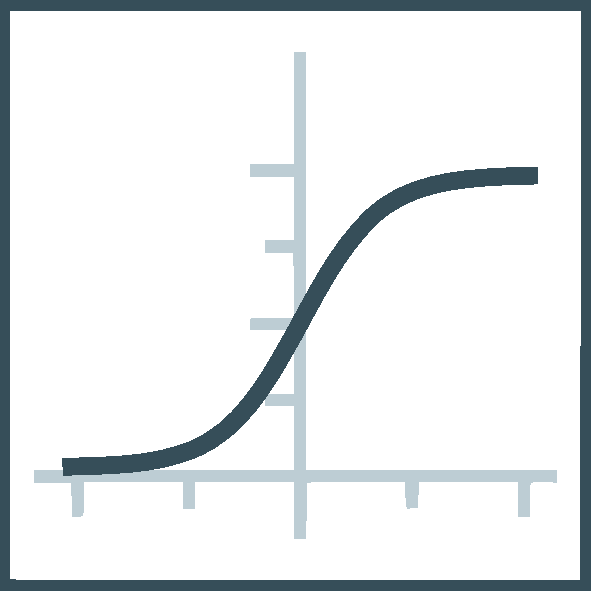
\includegraphics[width=2em]{images/sigmoid.pdf}
		\end{figure}
	};
	%\node [base] [left=-3em of brace]{%
	%	\begin{figure}
	%		
\includegraphics[width=3em]{images/ai.pdf}
	%	\end{figure}
	%};
\end{tikzpicture}%
